\section{Hasil menurut kelompok barang HS-6}\label{sec:goods}
\subsection{Gambaran agregat Indonesia menurut tujuh kelompok}
Disaggregasi barang memperlihatkan informasi yang tidak sama dengan hasil total. Tabel~\ref{tab:goodslr} melaporkan koefisien yang relevan untuk depresiasi: koefisien kurs pada ARDL dan koefisien partial sum negatif pada NARDL. Positif mengarah pada perbaikan ketika terjadi depresiasi, sedangkan negatif mengarah pada pemburukan. Kode kelompok mengikuti Tabel~\ref{tab:groups}.

\begin{table}[!htbp]\centering
\caption{Koefisien jangka panjang kelompok Indonesia--seluruh dunia}
{\small\setlength{\tabcolsep}{3pt}\renewcommand{\arraystretch}{1.15}
\begin{tabular}{p{0.05\linewidth}p{0.105\linewidth}p{0.1\linewidth}p{0.25\linewidth}p{0.1\linewidth}p{0.1\linewidth}p{0.07\linewidth}}
\toprule
\textbf{Kel.} & \textbf{Model} & \textbf{Koef.} & \textbf{CI nominal 95\%} & \textbf{p} & \textbf{BH} & \textbf{Status}\\
\midrule
G1 & ARDL & 0,865 & [-0,600; 2,330] & 0,241 & 0,463 & --\\
G1 & NARDL & 1,358 & [-0,832; 3,548] & 0,218 & 0,420 & --\\
G2 & ARDL & 2,026 & [0,198; 3,853] & 0,031 & 0,124 & L+D\\
G2 & NARDL & 4,580 & [2,301; 6,859] & \(<0{,}001\) & 0,004 & L\\
G3 & ARDL & 0,005 & [-1,248; 1,259] & 0,993 & 0,994 & --\\
G3 & NARDL & -1,621 & [-4,084; 0,842] & 0,192 & 0,380 & --\\
G4 & ARDL & -0,139 & [-6,905; 6,627] & 0,967 & 0,993 & --\\
G4 & NARDL & 7,851 & [-12,014; 27,716] & 0,431 & 0,587 & --\\
G5 & ARDL & 1,425 & [-1,754; 4,604] & 0,373 & 0,586 & --\\
G5 & NARDL & 1,589 & [-2,188; 5,365] & 0,402 & 0,578 & --\\
G6 & ARDL & -1,355 & [-1,998; -0,711] & \(<0{,}001\) & 0,004 & L+D\\
G6 & NARDL & -0,504 & [-2,145; 1,136] & 0,539 & 0,649 & --\\
G7 & ARDL & -2,040 & [-2,629; -1,451] & \(<0{,}001\) & \(<0{,}001\) & L+D\\
G7 & NARDL & -0,112 & [-1,134; 0,911] & 0,827 & 0,897 & L\\
\bottomrule
\end{tabular}
}\label{tab:goodslr}
\end{table}

\begin{figure}[!htbp]\centering
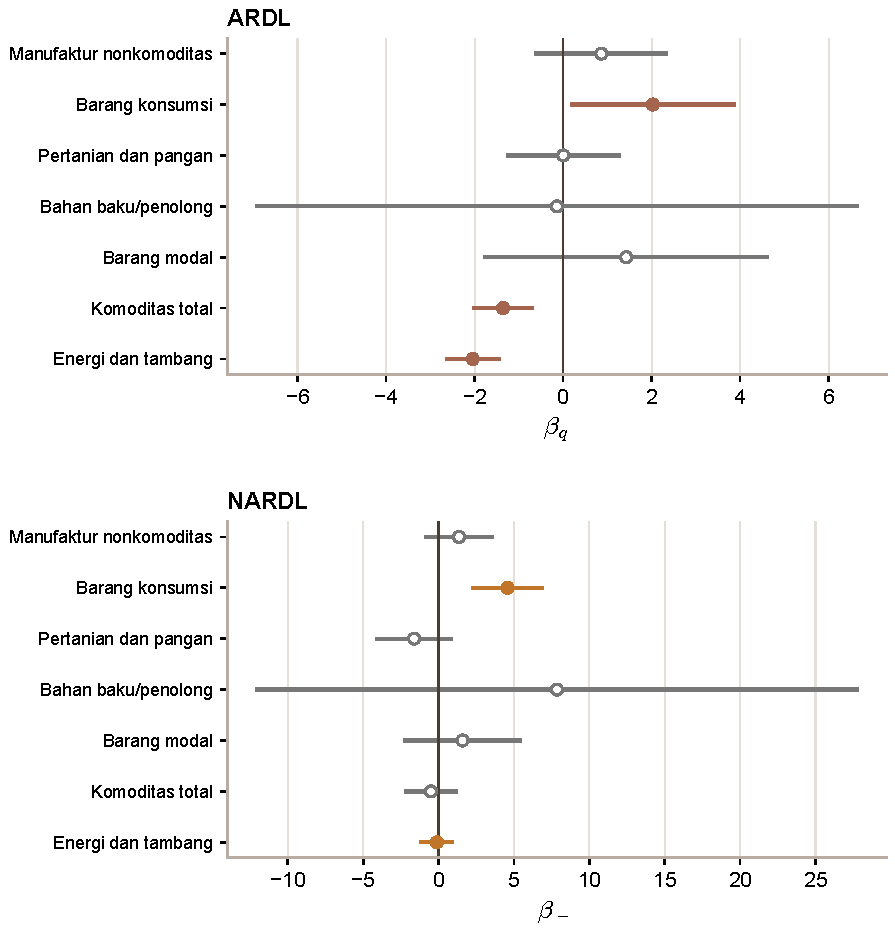
\includegraphics[width=\linewidth,height=.79\textheight,keepaspectratio]{assets/world_goods_forest.pdf}
\caption{Interval koefisien tujuh kelompok perdagangan Indonesia terhadap seluruh negara. Cokelat: syarat level dan diagnostik; emas: level dengan catatan diagnostik; simbol kosong: level belum lengkap. Status tidak menyatakan signifikansi koefisien dengan sendirinya.}\label{fig:goodsforest}
\end{figure}

Pada model linier, komoditas total dan energi/tambang memberikan koefisien negatif yang signifikan, dengan dukungan level serta diagnostik menurut aturan utama. Barang konsumsi mengarah positif dengan signifikansi nominal, tetapi nilai BH sekitar 0,124. Pada model nonlinear, barang konsumsi serta energi/tambang memenuhi syarat level, namun mempunyai catatan diagnostik. Tidak ada NARDL kelompok agregat yang sekaligus lolos syarat level dan seluruh penyaringan diagnostik yang digunakan.

\subsection{Komoditas total dan energi/tambang}
Koefisien ARDL komoditas total sekitar $-1,355$, dengan probabilitas nominal di bawah 0,001 dan BH sekitar 0,0037. Energi/tambang mempunyai koefisien sekitar $-2,040$ dengan probabilitas yang lebih kecil. Dengan orientasi apresiasi pada kurs, depresiasi berarti penurunan regressor; dikalikan koefisien negatif, perubahan outcome impor/ekspor mengarah positif atau memburuk.

Hasil ini relevan bagi hipotesis bahwa depresiasi tidak selalu memberi perbaikan. Namun ia belum mengidentifikasi apakah penyebabnya berada pada harga ekspor, volume, impor atau komposisi. Kelompok energi/tambang adalah bagian komoditas total, sehingga kedua temuan tidak boleh dihitung sebagai dua konfirmasi yang independen. Sebagian nilai perdagangan dan kejutan yang mereka alami sama.

NARDL memberikan gambaran lebih lemah untuk efek depresiasi kelompok tersebut. Koefisien komoditas total sekitar $-0,504$ tidak signifikan dan joint-X belum menolak meskipun F/t bounds menolak. Energi/tambang mempunyai koefisien depresiasi sekitar $-0,112$ yang tidak signifikan; hubungan level didukung, tetapi ada catatan heteroskedastisitas. Pada kelompok energi/tambang, Wald asimetri signifikan tidak berarti koefisien depresiasinya juga signifikan. Perbedaan koefisien kedua arah dan pengujian satu koefisien terhadap nol adalah pertanyaan berbeda.

\begin{figure}[!htbp]\centering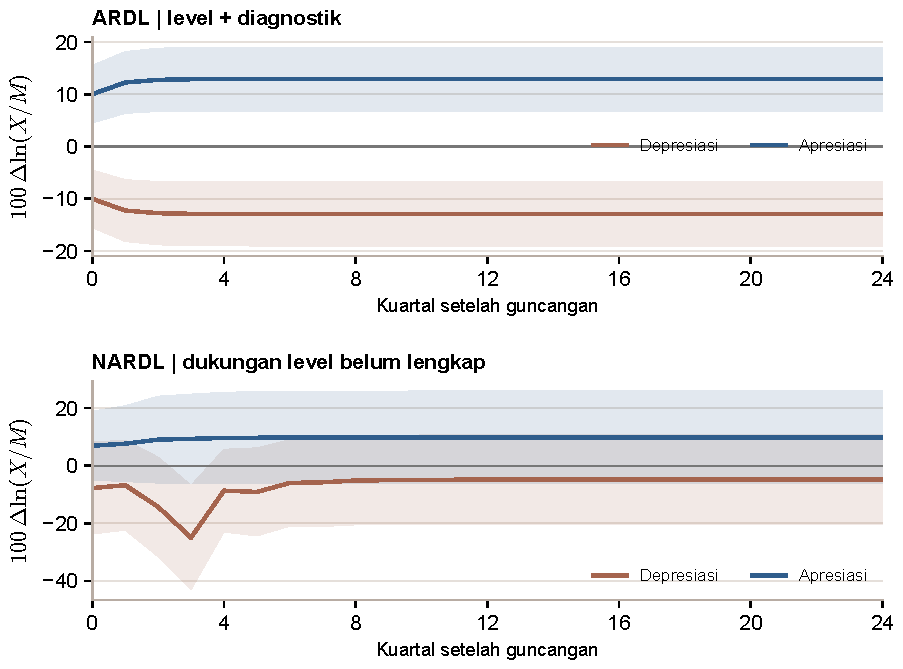
\includegraphics[width=\linewidth]{assets/response_TYPE_WLD_commodity.pdf}
\caption{Respons komoditas total Indonesia--seluruh dunia. ARDL mengarah pada pemburukan saat depresiasi; NARDL memberi ketepatan serta dukungan level yang berbeda. Band nominal pointwise 95\%.}\label{fig:commodity}
\end{figure}

\subsection{Manufaktur nonkomoditas}
ARDL manufaktur nonkomoditas memberi koefisien sekitar 0,865 dan NARDL koefisien depresiasi sekitar 1,358. Kedua probabilitas nominal berada di atas lima persen. Dukungan hubungan level juga belum lengkap. Karena itu, tanda titik positif belum dapat dipakai menyatakan bahwa manufaktur terbukti lebih diuntungkan oleh depresiasi dibandingkan komoditas.

Kegagalan menolak efek nol tidak sama dengan bukti bahwa efeknya kecil secara ekonomi. Interval harus cukup sempit untuk membedakan efek yang dianggap kecil dari yang relevan, dengan batas yang ditetapkan dan dijustifikasi. Run ini belum melakukan uji ekuivalensi tersebut. Membandingkan koefisien satu kelompok yang signifikan dengan kelompok lain yang tidak signifikan juga belum merupakan uji formal selisih dua koefisien.

\subsection{Konsumsi, pertanian, bahan baku/penolong dan modal}
NARDL konsumsi memberikan koefisien depresiasi sekitar 4,580, signifikan nominal maupun BH. Namun ada korelasi serial, heteroskedastisitas, RESET dan CUSUMSQ yang ditolak. Koefisien yang besar tidak dapat dipisahkan dari masalah spesifikasi ini. ARDL konsumsi lolos penyaringan utama dan memperlihatkan pola J pada titik, tetapi probabilitas BH-nya melewati lima persen dan dua fase belum terpisah kuat pada interval.

Pertanian/pangan dan modal memberikan contoh lain mengapa F/t tidak dibaca sendirian. Pada NARDL keduanya menolak no-level relation menurut F/t, tetapi joint-X belum mendukung. Bahan baku/penolong memberi interval yang sangat lebar dan catatan CUSUM, sementara syarat F/t juga belum lengkap. Tambahan parameter dan variasi regressor yang terbatas dapat mengurangi ketepatan. Koefisien besar pada kelompok ini karena itu tidak diperlakukan sebagai elastisitas yang telah mapan.

Klasifikasi penggunaan barang tidak mengaktifkan kembali hipotesis kandungan input impor. Besarnya koefisien bahan baku/penolong belum menjelaskan ketergantungan eksportir pada bahan asing. Data yang dibutuhkan untuk mekanisme itu berbeda dari pengelompokan perdagangan berdasarkan penggunaan barang.

\subsection{Perbedaan antara kelompok agregat dan kelompok bilateral}
Pertanian Indonesia--Tiongkok memberi contoh arah pemburukan yang lebih terukur pada NARDL. Koefisien depresiasinya sekitar $-2,037$, dengan probabilitas nominal sekitar 0,0016 dan BH sekitar 0,0148, serta memenuhi syarat level dan diagnostik utama. Temuan itu berlaku pada rasio neraca pertanian dengan Tiongkok dalam window model. Ia tidak menetapkan bahwa seluruh ekspor pertanian Indonesia menurun akibat depresiasi.

Sebaliknya, modal Indonesia--Korea dan konsumsi Indonesia--AS memberikan contoh urutan J yang lebih jelas pada band pointwise: ada bagian awal di bawah nol dan akhir horizon di atas nol. Kedua spesifikasi lolos penyaringan level dan diagnostik utama. Hal ini memperlihatkan bahwa bukti di dalam data tidak hanya mengarah pada satu sisi hipotesis. Tetap diperlukan kehati-hatian karena pencarian horizon, pemilihan AIC dan pengujian banyak kelompok belum tercakup dalam uji simultan seluruh jalur.

\begin{figure}[!htbp]\centering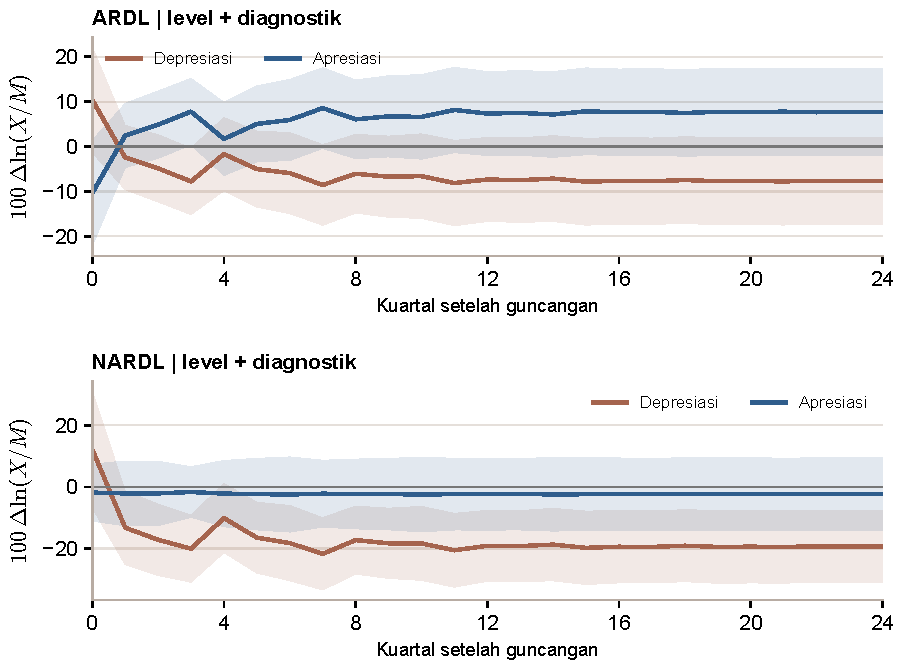
\includegraphics[width=\linewidth]{assets/response_TYPE_CHN_agriculture.pdf}
\caption{Pertanian Indonesia--Tiongkok sebagai contoh perbedaan hasil linier dan nonlinear. Positif berarti perbaikan rasio ekspor/impor.}\label{fig:chinaagri}
\end{figure}

Pada modal Korea, probabilitas BH koefisien depresiasi sekitar 0,104, sedangkan konsumsi AS sekitar 0,0027. Kejelasan dua fase pada band pointwise karena itu belum berarti semua koreksi pengujian berganda telah dilalui oleh keduanya.

\begin{figure}[!htbp]\centering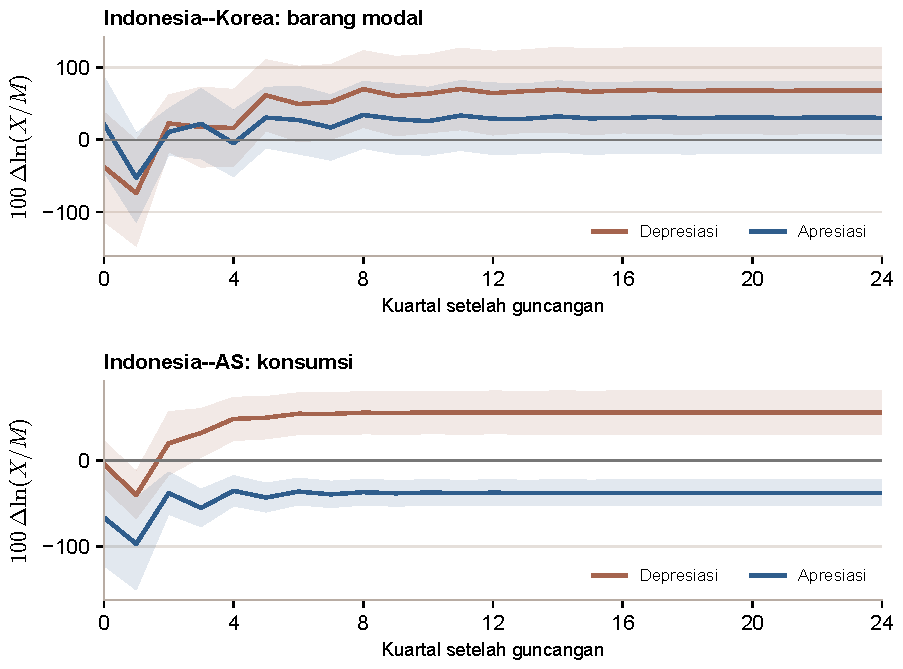
\includegraphics[width=\linewidth]{assets/J_examples.pdf}
\caption{Dua contoh NARDL dengan fase awal dan akhir yang lebih terpisah pada band pointwise: modal Indonesia--Korea dan konsumsi Indonesia--AS. Pemilihan horizon serta seleksi model belum tercakup dalam uji simultan.}\label{fig:Jexamples}
\end{figure}

Kesimpulan kelompok bersifat heterogen dan bergantung spesifikasi. Data memberi alasan melampaui satu angka agregat, tetapi belum mendukung penggantian generalisasi bahwa depresiasi selalu menguntungkan dengan generalisasi lain bahwa komoditas selalu tidak responsif atau selalu dirugikan.
